\documentclass[journal,hidelinks]{IEEEtran}
\usepackage[utf8]{inputenc}
\usepackage[
  pdftitle={Assignment \#2},
  pdfauthor={Andrei Purcarus},
  pdfsubject={ECSE-526 -- Artificial Intelligence}
]{hyperref}
\usepackage{graphicx}
\usepackage[all]{hypcap}
\usepackage{cleveref}
\usepackage{indentfirst}
\usepackage[per-mode=symbol]{siunitx}

\title{ECSE-526 \\ Artificial Intelligence \\ Assignment \#2}
\author{Andrei~Purcarus,~260631911,~\IEEEmembership{McGill~University}}

\begin{document}
\sloppy

\maketitle

\begin{abstract}

An agent capable of classifying songs into 10 genres (classical, country, edm dance, jazz, kids, latin, metal, pop, rnb, and rock) was created and tested using cross-validation. Several methods of classification were tried, such as a Gaussian classifier, a k-nearest neighbours (kNN) classifier, and a random decision forest classifier. Cross-validation showed that the kNN classifier with $k = 1$ was the best classifier for the given task of music classification.

\end{abstract}

\section{Introduction}

\IEEEPARstart{T}{his} report describes the creation of an agent capable of classifying songs into one of 10 genres (classical, country, edm dance, jazz, kids, latin, metal, pop, rnb, and rock).
To achieve this goal, we were provided with data in the form of a set of 12-dimensional floating point feature vectors for each song. In addition, we were provided with labels classifying each song with the correct genre.
The goal was therefore to use this data to train an agent that can classify the songs in a test set as accurately as possible.
We first describe the creation of a Gaussian classifier and present an analysis of its expected performance. We also look at the underlying assumptions we make when we model the data using a Gaussian normal distribution.
Then, we describe a k-nearest neighbours (kNN) classifier and look at the values of k for which this classifier works best.
Next, we describe the other types of classifiers that we implemented.
Finally, we compare the performance of each classifier using cross-validation to find the one best suited to the task of music classification.

\section{Gaussian Classifier}
\label{sec:gauss}

First, we implemented a Gaussian classifier. In this classifier, training consists of grouping all the training data by genre and computing the average vector and covariance matrix for each set. Then, to classify new feature vectors, we use the unnormalized log likelihood to compute a measure of how closely the feature vector fits into each genre's normal distribution. Given an average vector $\mu$ and a covariance matrix $\Sigma$, we thus find the genre $i$ with the minimum value of
\[ UNLL_{i} = (x - \mu_{i})^T \Sigma_{i}^{-1} (x - \mu_{i}) \]

We implemented two versions of this model. The first one, which we call the Gaussian classifier, takes the set of averages of each song's features as the training set. When it has to classify a new song, it computes the average feature vector for said song and compares it to the normal distributions of the averages of other songs. The second model, which we call the Total Gaussian classifier, uses the raw feature vectors to compute the normal distribution for each genre and then classifies new songs by first classifying all their feature vectors and then taking the plurality vote among the results.

In using this model, we make several assumptions about the data. We assume that the feature vectors for each genre are produced by a single statistical model. In addition, we assume that this model is one in which features are normally distributed around a mean value. Essentially, this means that we assume each genre has a "true" value, with Gaussian noise spreading the data around that point. In addition, we assume that the data points are independent. This last assumption, combined with the fact that feature vectors within a song might be correlated, helps explain why the Gaussian classifier performs so much better than the Total Gaussian classifier during cross-validation (\Cref{tab:results}): By taking the average feature vector for each song, it better satisfies the third assumption of independence.

With these three assumptions in mind, we can see where we might expect the Gaussian classifier to perform well and where it might fall short. In situations such as classifying factory parts into different types, where the parts can be modeled as ideal parts with manufacturing error that is normally distributed, a Gaussian classifier can be expected to perform very well. However, there are many situations where the model can perform poorly. One such situation is where the data for a class actually consists of many local clusters of data points at different locations. Then, the average will have nothing to do with the actual distribution of the data, and a nearest neighbour approach will likely outperform it since it uses a more local classification method. Another example where the Gaussian fails is when two classes have the same averages. Then, the UNLL will depend only on the covariance matrix. Thus, a class with a strictly greater covariance matrix will always be chosen over one with a smaller one.

\section{K-Nearest Neighbours Classifier}
\label{sec:knn}

Next, we implemented two types of kNN classifiers. One is the standard kNN classifier that selects the prediction based on a plurality vote of the k nearest neighbours. The other is a weighed kNN classifier that assigns to each nearest neighbour a weight $w = 1 / d^2$, where $d$ is the distance between the feature vector to be classified and the neighbour. It then normalizes these weights for each feature vector and averages them over all feature vectors in a song to make a prediction.

In order to speed up predictions, we used two different implementations of a KD tree. One is a standard KD tree that splits the data into two equal sets at each node such that one set has lower values than a threshold for a given feature and the other has higher values. Search can then be sped up by eliminating subtrees that cannot contain nearest neighbours. The other is an implementation of a best bin first KD tree that uses a priority queue to keep track of which nodes to visit next. This approach visits closer nodes sooner, and thus it lends itself to early cutoff with much better results \cite{beis_shape_1997}.

As shown in \Cref{tab:results}, the best value of $k$ found during experimentation was $k = 1$ for both the standard and weighed implementations. For standard kNN, the performance experiences a peak at $k = 1$, then drops drastically and starts climbing back up slowly as $k$ increases. A possible explanation of this phenomenon is that the nearest neighbours are evenly distributed among genres. When a single neighbour is used, it will always be the nearest one that classifies a feature vector. With $k = 3$, if the three neighbours disagree the prediction will choose a random classification among the three. As $k$ increases, the presence of more neighbours allows the predictions to reach an actual plurality and improves the accuracy. With weighted selection, we can see that the results are more normalized since more distant neighbours contribute less to the prediction.

\section{Other Classifiers}

We also implemented a classifier called the random decision forest classifier. In this type of classifier, $N$ decision trees are each trained on a subset of the data and a subset of the features. These subsets are randomly chosen with replacement. In our implementation, we used sizes of $2 * D / 3$ and $2 \sqrt{F}$, respectively, where $D$ is the total number of training examples and $F$ is the total number of features. The forest then selects the best prediction based on a plurality vote of the trees. The trees themselves were built by splitting the data at each node into two subsets based on whether they lie above or below a threshold value for a given feature. All such splits are tried for each randomly selected feature and the one that minimizes entropy is selected.

\section{Results}

To evaluate the different classifiers, we used a cross-validation method where the training data was randomly split into 10 subsets of equal size. Then, the classifiers were allowed to train on 9 of these subsets and tested against the 10th. This process was repeated for each possible 9-1 split and the results were averaged to give a final performance metric. The results are plotted in \Cref{fig:results}, with the corresponding data shown in \Cref{tab:results}. Note that to speed up the search, a best bin first KD tree was used for both kNN and weighed kNN with a cutoff set at $400 * k$ leaf nodes.

\begin{figure}[!htb]
  \centering
  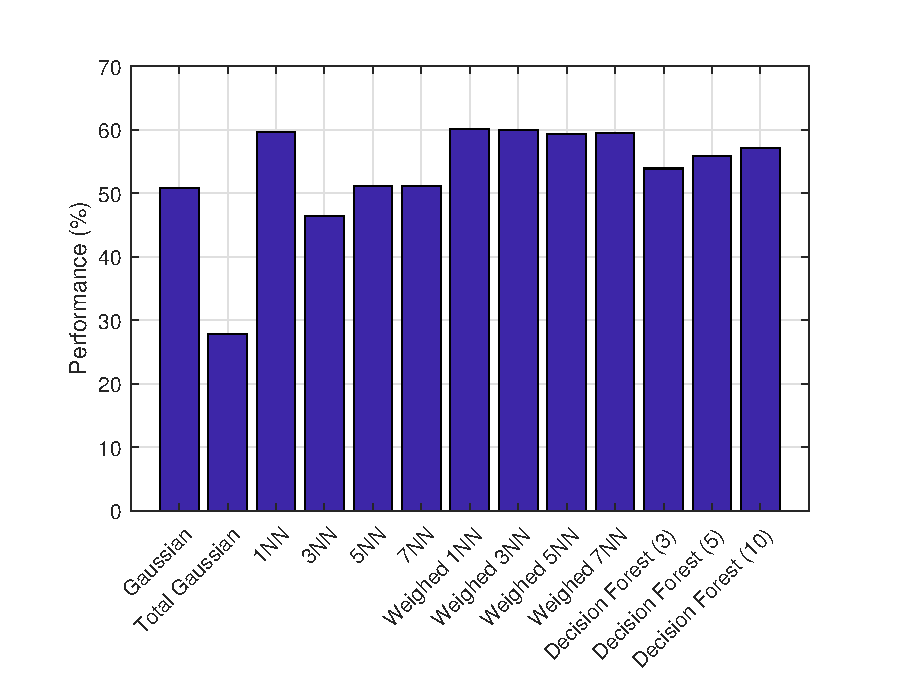
\includegraphics[width=\columnwidth]{cross_validation.eps}
  \caption{Cross-validation results for the implemented music classifiers.}
  \label{fig:results}
\end{figure}

\begin{table}[!htb]
	\centering
	\caption{Cross-validation results for the implemented music classifiers.}
	\label{tab:results}
	\resizebox{0.8\columnwidth}{!}{\begin{tabular}{l|l}
		\textbf{Classifier} & \textbf{Performance (\%)} \\ \hline
		Gaussian & 50.8 \\
		Total Gaussian & 27.8 \\
		1NN & 59.6 \\
		3NN & 46.4 \\
		5NN & 51.2 \\
		7NN & 51.2 \\
		Weighed 1NN & 60.2 \\
		Weighed 3NN & 60.0 \\
		Weighed 5NN & 59.3 \\
		Weighed 7NN & 59.5 \\
		Decision Forest (3) & 53.9 \\
		Decision Forest (5) & 55.8 \\
		Decision Forest (10) & 57.2 \\
	\end{tabular}}
\end{table}

From these figures, it is clear that the kNN and weighed kNN classifiers are the best at classifying music genres, followed closely by the random decision forest, then the Gaussian, and finally the Total Gaussian.

The fact that the nearest neighbour approach is the best classifier for this data set can be seen as an indicator that feature vectors for a genre tend to cluster together such that they are close to other members of the same genre. We looked at the best values of $k$ back in \Cref{sec:knn}.

The next best performer, the random decision forest, can be viewed as similar to the nearest neighbour classifiers, since a decision tree cuts up the N-dimensional space into local subspaces and assigns each subspace a genre. It is therefore more coarse than kNN since it lumps together groups in the same subspace. In fact, we can see from \Cref{fig:results} that the decision forest performance increases with the number of trees. Therefore, we might reasonably expect that with sufficient trees, its performance might exceed that of the kNN. One additional thing to keep in mind is that the trees were not pruned. Given pruning, the forest might perform even better by reducing the extent of overfitting for individual trees.

As mentioned in \Cref{sec:gauss}, the poor performance of the Total Gaussian classifier can be explained by the correlation present between feature vectors in the same song, which violates our assumptions in modeling the data as a Gaussian distribution. Indeed, we can see that when we average the feature vectors for each song, we get almost twice the performance out of a Gaussian classifier. Even so, the kNN outclasses the Gaussian classifier, indicating that the data is better represented by local clusters than a global normal distribution.

\section{Conclusions}

In conclusion, we created an agent capable of classifying songs into 10 genres and tested it using cross-validation. We tried several classification methods including the Gaussian classifier, the kNN classifier, and the random decision forest classifier. We then found that the kNN classifier with $k = 1$ is the best classifier for the given task of music classification.

\bibliographystyle{IEEEtran}
\bibliography{IEEEabrv,references}

\end{document}
